\documentclass[draft=True]{thesis}
\usepackage{graphicx, slashed, siunitx}
\usepackage[utf8]{inputenc}
\usepackage{xr-hyper}
\documentclass[a4paper,10pt,draft]{thesis}
\usepackage{physics,amsmath, amsfonts, siunitx, amssymb, graphicx, slashed,subcaption}
\usepackage[utf8]{inputenc}
\usepackage[margin=1in]{geometry}
\usepackage[hidelinks]{hyperref}
\usepackage{xr-hyper}
\newcommand{\n}[1]{\nu_{#1}}
\newcommand{\na}{\nu_\alpha}
\newcommand{\nb}{\nu_\beta}
\newcommand{\ana}{\bar{\nu}_\alpha}
\newcommand{\an}[1]{\bar{\nu}_{\text{#1}}}
\newcommand{\anb}{\bar{\nu}_\beta}
\renewcommand{\a}{\alpha}
\renewcommand{\b}{\beta}
\newcommand{\ab}{\alpha\beta}


\renewcommand{\ne}{\nu_e}
\newcommand{\nm}{\nu_\mu}
\newcommand{\nt}{\nu_\tau}
\newcommand{\ns}{\nu_s}

\newcommand{\ane}{\bar{\nu}_e}
\newcommand{\anm}{\bar{\nu}_\mu}
\newcommand{\ant}{\bar{\nu}_\tau}
\newcommand{\ans}{\bar{\nu}_s}

\newcommand{\nee}{\nu_e \to \nu_e}
\newcommand{\nem}{\nu_e \to \nu_\mu}
\newcommand{\net}{\nu_e \to \nu_\tau}
\newcommand{\nes}{\nu_e \to \nu_s}

\newcommand{\nme}{\nu_\mu \to \nu_e}
\newcommand{\nmm}{\nu_\mu \to \nu_\mu}
\newcommand{\nmt}{\nu_\mu \to \nu_\tau}
\newcommand{\nms}{\nu_\mu \to \nu_s}



\newcommand{\Pee}{P_{e  e}}
\newcommand{\Pem}{P_{e  \mu}}
\newcommand{\Pet}{P_{e  \tau}}
\newcommand{\Pes}{P_{e  s}}

\newcommand{\Pme}{P_{\mu  e}}
\newcommand{\Pmm}{P_{\mu\mu}}
\newcommand{\Pmt}{P_{\mu  \tau}}
\newcommand{\Pms}{P_{\mu  s}}


\newcommand{\Pte}{P_{P_{\tau e}}}
\newcommand{\Ptm}{P_{\tau  \mu}}
\newcommand{\Ptt}{P_{\tau  \tau}}
\newcommand{\Pts}{P_{\mu  s}}

\newcommand{\Paeae}{P_{\bar{e}  \bar{e}}}
\newcommand{\Paeam}{P_{\bar{e}  \bar{\mu}}}
\newcommand{\Paeat}{P_{\bar{e}  \bar{\tau}}}
\newcommand{\Paeas}{P_{\bar{e}  \bar{s}}}

\newcommand{\Pamae}{P_{\bar{\mu}  \bar{e}}}
\newcommand{\Pamam}{P_{\bar{\mu}  \bar{\mu}}}
\newcommand{\Pamat}{P_{\bar{\mu}  \bar{\tau}}}
\newcommand{\Pamas}{P_{\bar{\mu}  \bar{s}}}


\newcommand{\Patae}{P_{\bar{\tau}  \bar{e}}}
\newcommand{\Patam}{P_{\bar{\tau}  \bar{\mu}}}
\newcommand{\Patat}{P_{\bar{\tau}  \bar{\tau}}}
\newcommand{\Patas}{P_{\bar{\mu}  \bar{s}}}

\renewcommand{\th}[1][]{%
  \theta\ifx\\#1\\\else_\text{#1}\fi
}
\newcommand{\thm}[1][]{%
  \theta^\text{M}\ifx\\#1\\\else_\text{#1}\fi
}
\renewcommand{\t}[1]{\text{{#1}}}
\newcommand{\avg}[1]{\left\langle {#1} \right \rangle}
\newcommand*{\dm}[1][]{%
  \Delta m^2\ifx\\#1\\\else_\text{#1}\fi
}
\newcommand{\zreco}{\cos{(\theta_z^{reco})}}
\newcommand{\ztrue}{\cos{(\theta_z^{true})}}
\newcommand{\z}{\cos{(\theta_z)}}
\newcommand{\Ereco}{E^{reco}}
\newcommand{\Etrue}{E^{true}}
\newcommand{\Aeff}{A^\text{eff}}
\newcommand{\emm}{\epsilon_{\mu\mu}}
\newcommand{\emt}{\epsilon_{\mu\tau}}
\newcommand{\eet}{\epsilon_{e\tau}}
\newcommand{\eem}{\epsilon_{e\mu}}
\newcommand{\ett}{\epsilon_{\tau\tau}}
\newcommand{\ep}{\epsilon^\prime}

\begin{document}
We always observe neutrinos indirectly through their associated charged lepton. Regardless of the type of interaction (charged current via the $W$ boson, or neutral current
via the $Z$), a charged lepton exits with altered properties. The lepton is then detected, and the properties of the neutrino involved in the 
interaction is then deduced. This deduction is obviously imperfect, and this introduces complexities that we will handle in Ch.~\ref{ch:ICmethod}. 

In this work, we only study the detectors handeled by the ICecube collaboration. They are of Cherenkov type, which means that they detect 
the charged lepton by its emitted Cherenkov light, produced from its travel through the Antarctic ice. 
%TODO: text about pid
\begin{figure}\label{fig:events}
    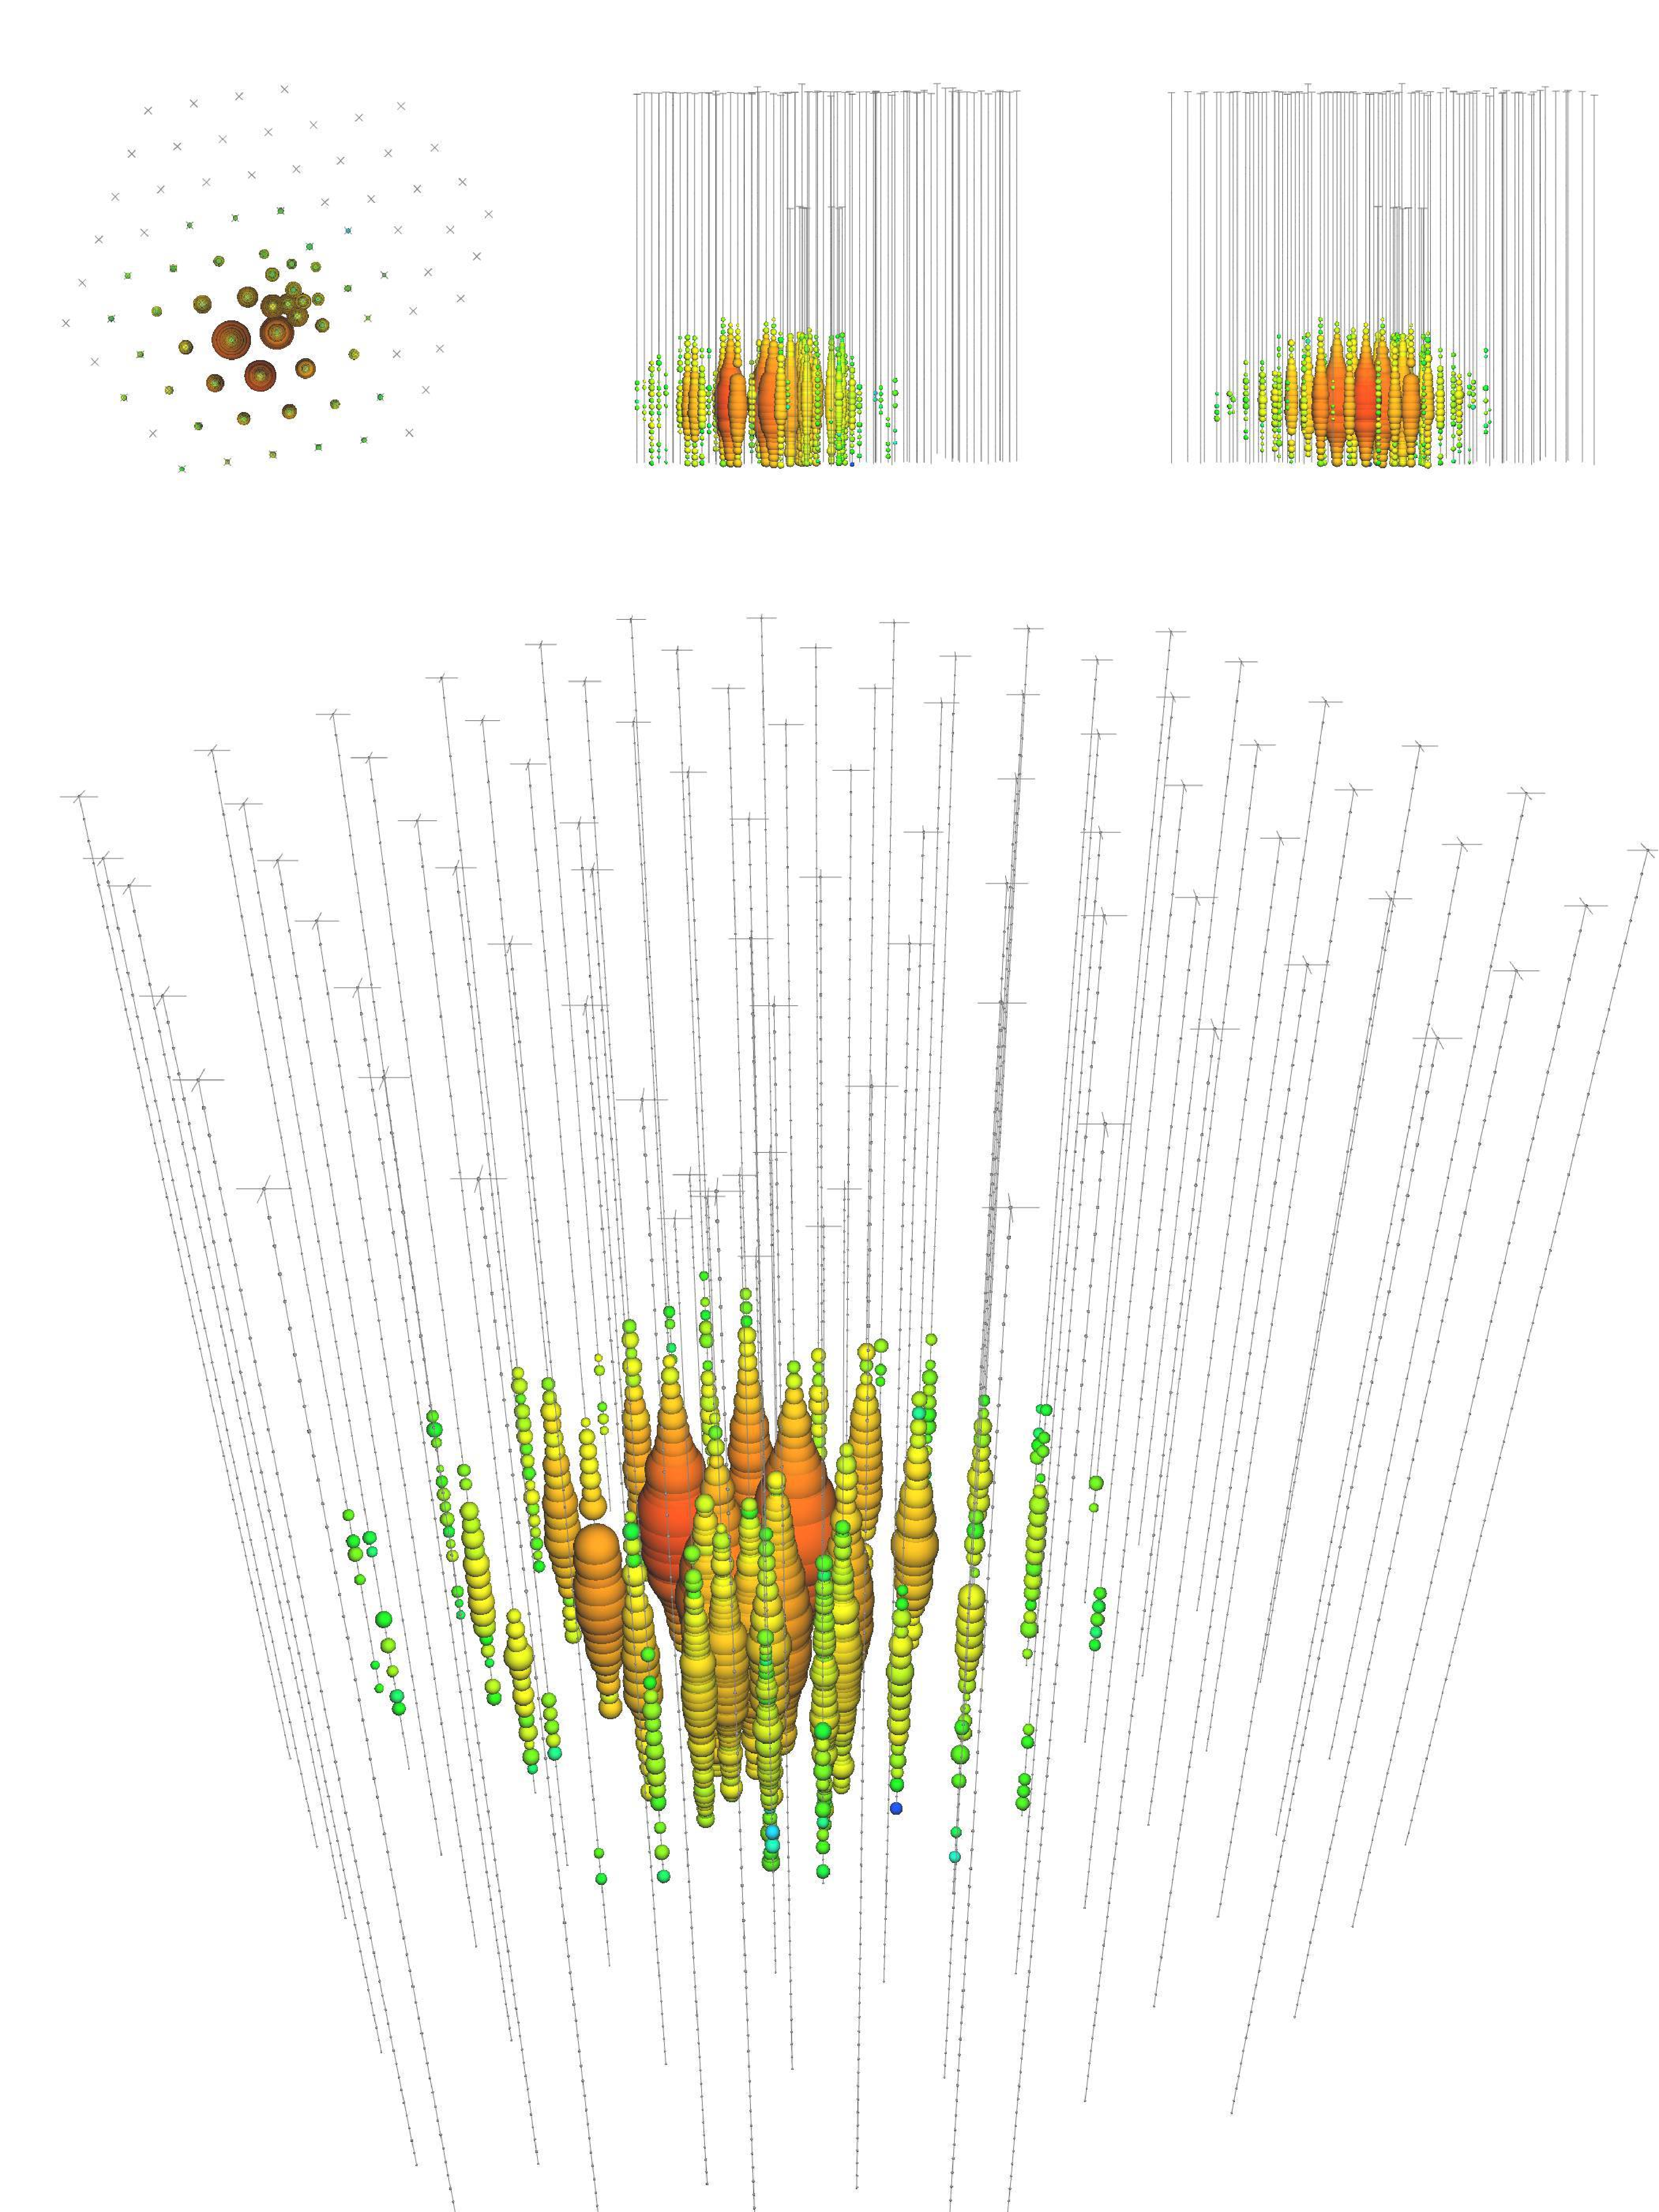
\includegraphics[width=0.5\textwidth]{figures/cascade_event.pdf}\caption{Event classified as cascade}
    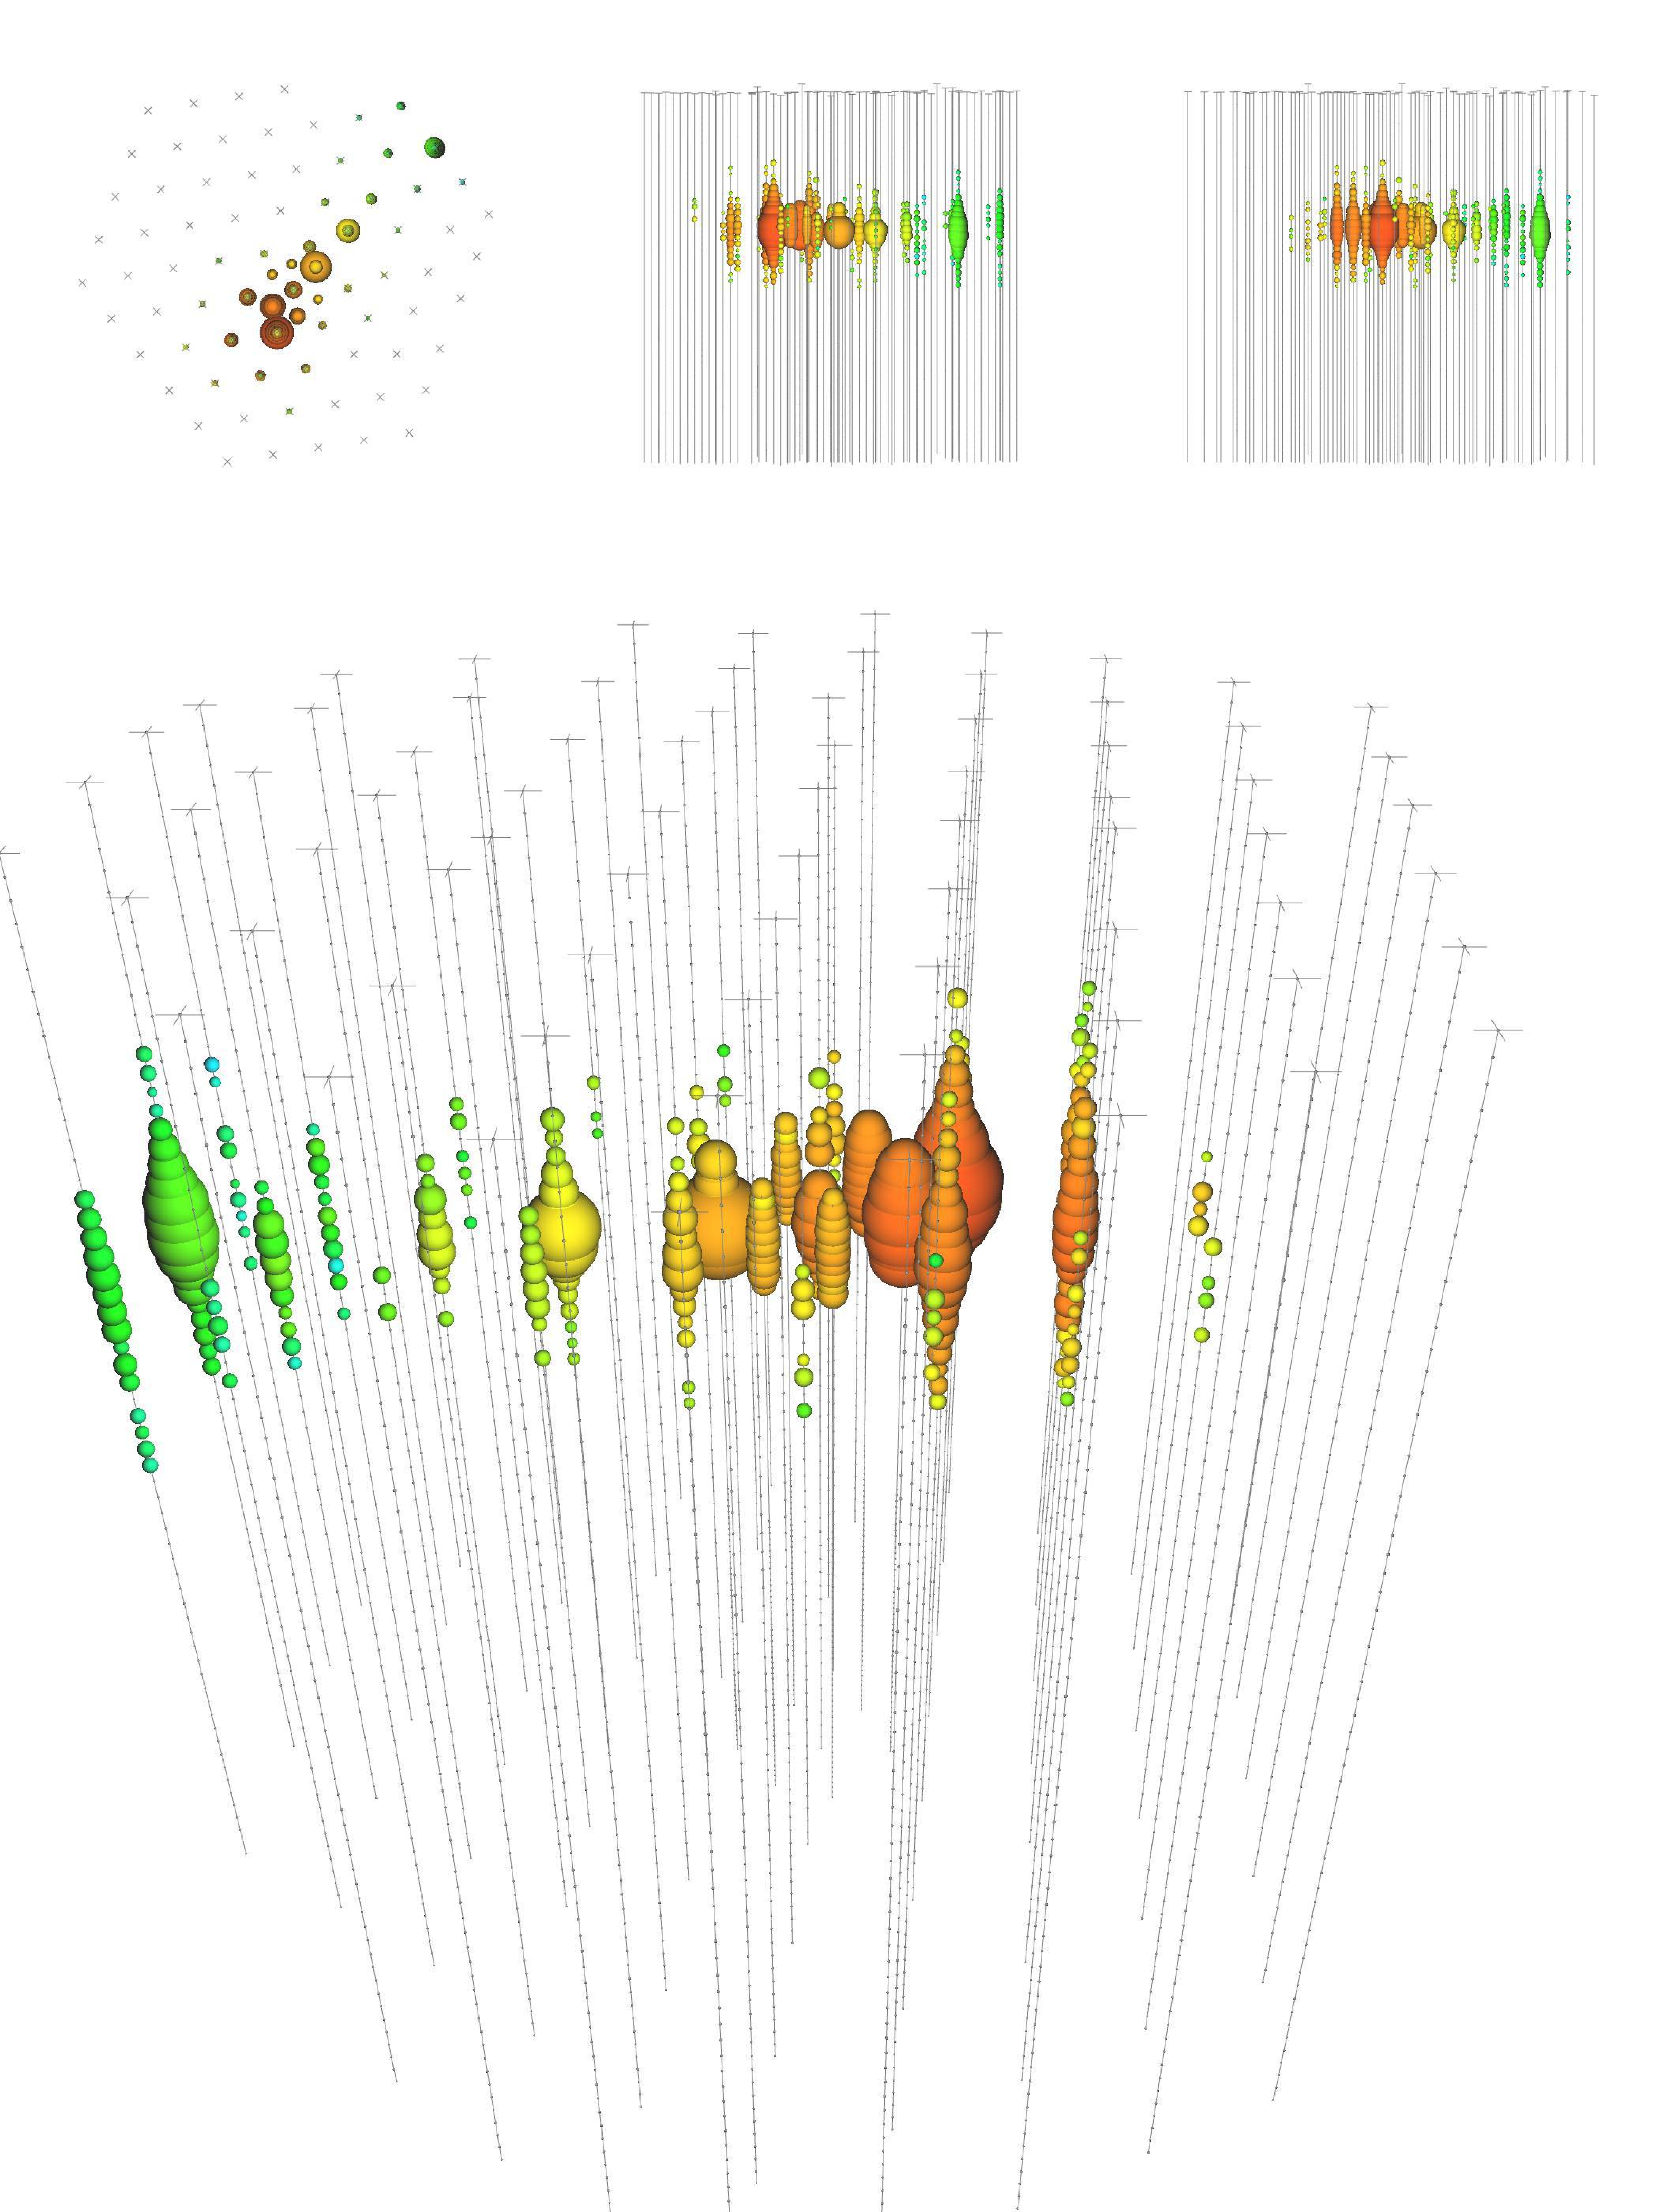
\includegraphics[width=0.5\textwidth]{figures/track_event.pdf}\caption{Event classified as track}
\end{figure}

To detect the Cherenkov light, 60 Digital Optical Modules (DOMs) are placed on a long string up to \SI{17}{\metre} apart. 86 of these strings are then lowered
into \SI{2.5}{\km} deep boreholes in the ice. The holes are then sealed by refreezing the ice, resulting in a total of 5160 DOMs in a volume of approximately \SI{1}{\km^3}~\cite{weaverThesis}.
%TODO: pic of cherenkov light/dom?

The strings and DOMs are not spaced evenly, making some parts of the detector more sensitive to certain energy ranges than other.
8 strings packed more tightly than the other 78, making that part of the detector sensitive to neutrino energies down to single digit \si{\GeV}. Due to 
this part being situated deep within the ice, it is referred to DeepCore. DeepCore will be treated as a separate and independent detector from the rest, which
retains the name IceCube. A view of the current setup can be seen in Fig.~\ref{fig:array}. In this work, we consider DeepCore data between \SIrange{5.6}{56}{\GeV} and IceCube data in the range \SIrange{0.5}{10}{\TeV}.
\begin{figure}\label{fig:array}
    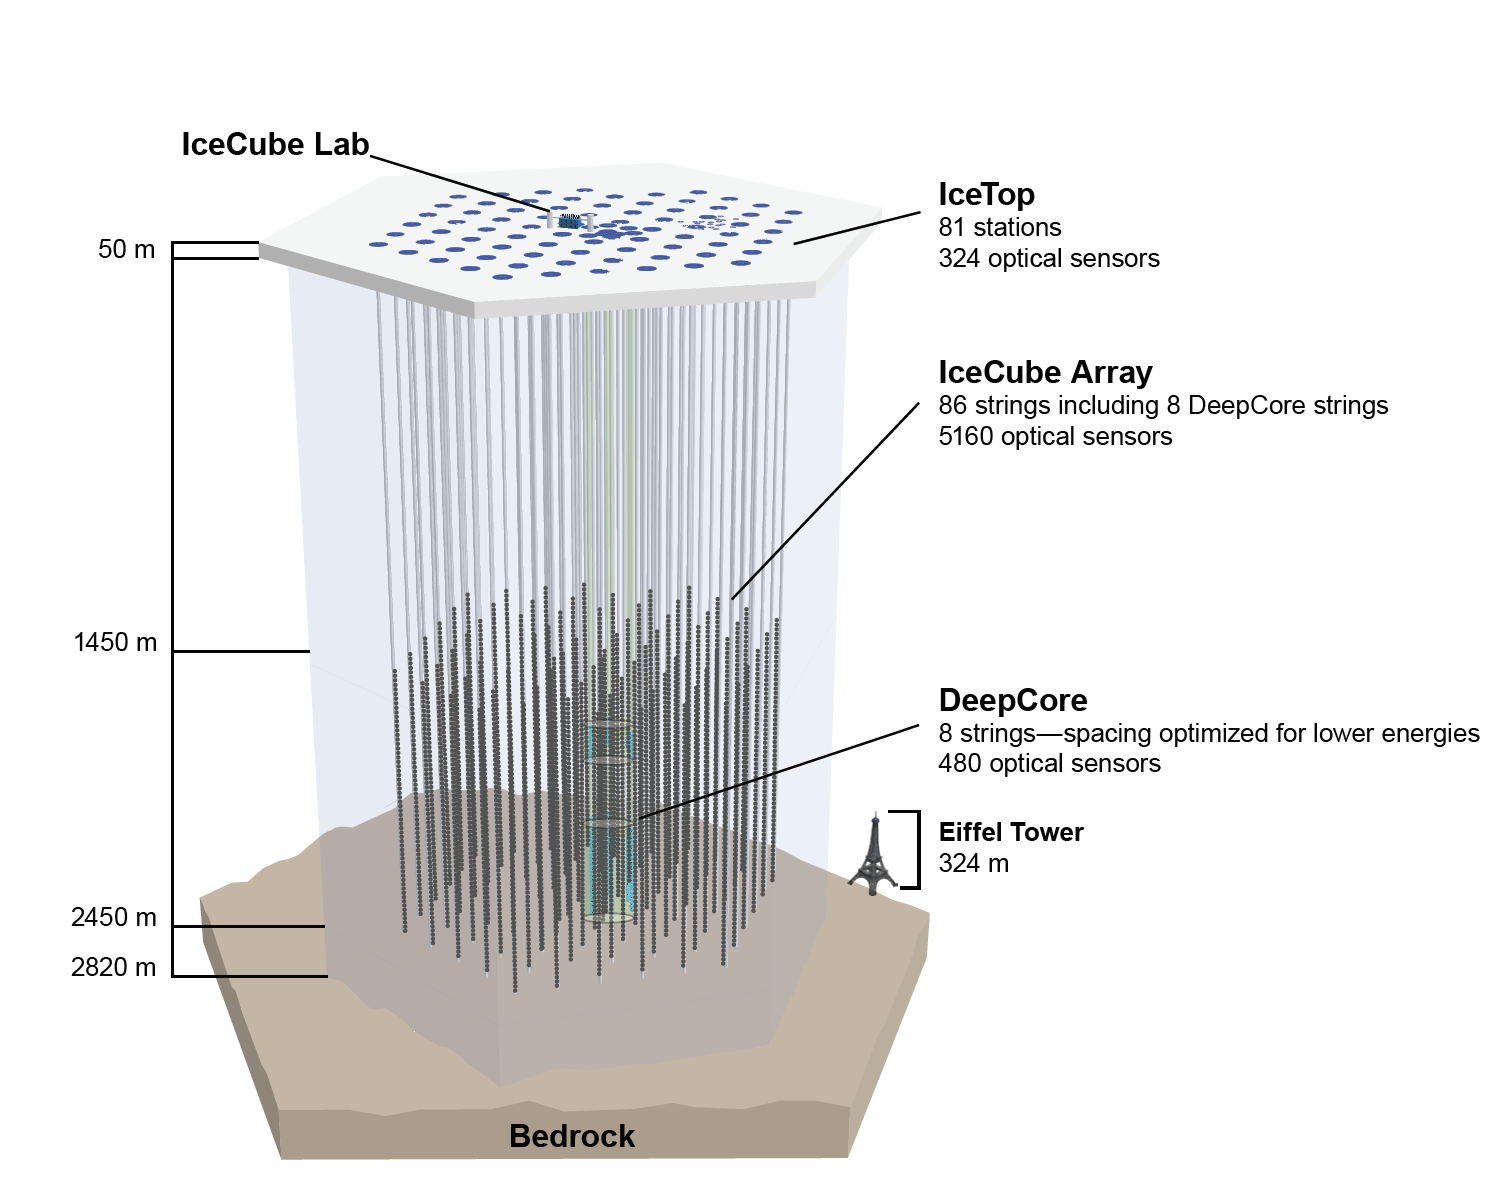
\includegraphics[width=0.5\textwidth]{figures/icecube2.png}\caption{View of the full IceCube array}
\end{figure}

In 2017, the PINGU Letter of Intent was published~\cite{PINGUletter}. The "Precision IceCube Next Generation Upgrade" is an upgrade that will 
supplement DeepCore, i.e. boosing the capabilites of neutrino detection at the \si{\GeV} scale. As the PINGU upgrade is not yet financed nor built, we are
not able to use any data from it. However, the collaboration has released preliminary simulations which we will use to see how the upgrade might improve
IceCube and DeepCore bounds. 
\bibliographystyle{nature}
\bibliography{ref.bib}
\end{document}